\chapter{State selective light shifts for spin-sensitive imaging}%
\label{ch:spin_resolved}
%\subsection*{General idea and length}

%\begin{itemize}
%\item Explain problem, that is: No idea which spins are occupying the tweezers. (1 page)
%\item Reference back to aod setup and explain that we use the same tweezers to select the spins (1-2 pages)
%\item Theory about spin selecting, could also say something about the first idea that didn't work out (2-4 pages)
%\item Explain in full detail the laser setup (1-2 pages)
%\item Show laser curve, maybe laser diode specs (1-2 pages)
%\item Then all the cavity stuff, which is how we built it and why we decided to use the materials. (4-5 pages)
%\item Then show drift measurements, explaining how beating works (1-2 pages)
%\item Conclude with outlook on building it in? (1-2 pages)
%\end{itemize}

Being able to measure the spin of ground state potassium atoms in many-body quantum experiments gives insight into the full quantum state and thus being able to pinpoint the ground state on the Bloch sphere. In Rydberg dressing experiments~\cite{Bouchoule2002, Pupillo2010, VanBijnen2015, Glaetzle2015, Zeiher2016, Borish2020}, where the atom is in a ground state and fractionally in an excited Rydberg state, the spin can be used in a Ramsey sequence, in order to measure correlations~\cite{Zeiher2017}.
This is, since the ground state atoms in a superposition of two spins, couple to the Rydberg state. To measure effects, such as Rydberg blockade~\cite{Jaksch2000, Urban2009}, and the resulting correlations, the superposition state acquires a phase on the Bloch sphere, which needs to be evaluated. This is currently achieved, by doing a projection measurement by removing one component out of the system.

With the new approach, it is possible to evaluate the spin species, by separating them in independent tweezers. A spin-sensitive tweezer array is then moved, and thus the atoms having this spin component follow this dipole potential. This creates a separation, and by evaluating the geometry from a fluorescence image, it is thus possible to find how the tweezer arrays were previously occupied. Measuring the spins this way, also means the atoms will not heat out during the process, and therefore the system can be reassembled and reused for further investigation.

The following chapter will discuss the setup in question in more detail, as well as the wavelength in use, in order to have tweezers sensitive to only one spin component. The new laser system is explained in detail, which includes a cavity for frequency stabilization, and therefore stability of the laser is discussed.

\section{Approaches}

Measuring the spin means in our experiment, to take a fluorescence image of the two ground states $F=1$ and $F=2$. However, during imaging, the spins are mixed, such that they can't be distinguished. As it was shown in Chapter~\ref{sec:sorting}, it is possible to move selected tweezers. Therefore two approaches are discussed in the following, both work by separating the two spins spatially, which requires finding ways of being sensitive to one specific ground-state spin. The first idea is using strong magnetic fields to increase the separation of the spin levels with the Zeeman effect. The second approach is using a state selective light shift, given by selecting a particular wavelength. This allows one spin component to be trapped, while the other will not see a trapping effect. In both applications, the idea is to trap one spin state in its own trap and physically move it away from the other. By taking an image, it is then possible to map positions to spins and therefore find out which tweezers contained which spin species. Moving the spin-sensitive tweezers back into its original position, the initial system is the reassembled and new measurements can be taken with more information.

\subsection{Zeemann induced potential separation}

Although the spin levels are too close in energy space, to address them  with imaging lasers, having a position dependent potential, that is different for each spin state, is enough to spatially separate them. One way of achieving this, is by applying magnetic fields. In 1896, Pieter Zeeman wrote about how magnetic fields were affecting spectroscopy of atoms~\cite{Zeeman1896}. From this followed the Zeeman effect, which explains how spectral lines of atoms are split and shifted when applying magnetic fields. This can be calculated perturbatively~\cite{Griffiths2004}, by modelling the atom as a magnetic dipole. In analogue to the classic description of magnetic dipoles, this gives an energy $V_M$ depending on the magnetic field $\bm{B}$:

\begin{align}
	V_M = - \bm{\mu} \bm{B}
\end{align}

and is then the perturbation in the total Hamiltonian $H = H_0 + V_M$. The magnetic moment $\bm{\mu}$ contains contributions from nuclear and electron spin, which then give direction and length of the magnetic dipole. The energy associated with the perturbation evaluates to

\begin{align}
	E_z = B_z \mu_B \left(g_l m_l + g_s m_s\right).
\end{align}

It has contributions from the nuclear spin ($g_l m_l$) and electron spin ($g_s m_s$) and depends on the Bohr magneton $\mu_B$. The magnetic quantum numbers $m_i, i\in\{l,s\}$ depend on the value of the associated quantum numbers, which are the orbital angular momentum $L$ and electron angular momentum $S$, such that $m_l \in \{-L, -L+1, \ldots, L-1, L\}$ and $m_s \in \{-S, -S+1, \ldots, S-1, S\}$. This means, not only is the hyperfine state shifted by the magnetic field, it is also split into more energy sublevels. However, a complete description of the energy shift, needs to integrate the shifts of the hyperfine levels, which has been done in the Breit-Rabi model~\cite{Breit1931}.

Figure~\ref{fig:pot_zeeman} gives an illustration of how the two spin components $F=1$ and $F=2$ in the potassium ground state are affected due to a magnetic field. Visible is a splitting of the spin-states into sublevels. In order to maximally separate the spin states, the $F=1$ spin would be pumped into the $m_F=1$ state, and consequently, $F=2$ into the $m_F=2$ state.

%The experiment is already able to generate a magnetic field of $\SI{40}{\gauss}$ with the use of the \ac{mot} coils, which are used to trap and cool the atoms initially. At this field strength, the separation is almost $\SI{600}{\mega\hertz}$.

Using this, the idea is to create a position dependent trap for the two spin-states. To do this, we need to note, that from the figure, the $F=1, m_F=1$ state has a negative slope, while the $F=2, m_F=2$ state has a positive slope. This means, simply by generating a magnetic field ramp, the atoms in different spin states, will see a position dependent energy $V_{mag}$. Since the atoms are trapped inside optical tweezers, the potential given by the dipole force is~\cite{LeKien2013}:

\begin{align}
	V_{dip}(r) = -\frac{\pi c^2 \Gamma}{2 w_0^3 \Delta} I(r),
\end{align}

where $\Gamma$ is the line width of the transition, in this case the D2 line, $\Delta$ the detuning, $w_0$ the resonance frequency and $I(r)$ the intensity of the laser beam. By applying the magnetic field gradient, the atoms see a total potential $V(r)$:

\begin{align}
	V(r) = V_{dip}(r) + V_{mag}(B(r)),
\end{align}

where the position dependence was explicitly noted. This way, the potential minimum, which was originally just given by the dipole trap, is now shifted in the direction of the potential induced by the Zeeman effect. Thus, the two spin states will see different potentials, which are shifted in position space with respect to each other. However, numerical calculations of the potential minimum show that the shift is too small in order to spatially separate the atoms. For this, it is assumed, the atom is trapped on the D2-line and the laser power is $\SI{1}{\micro\watt}$, where the spatial separation is favorable towards lower laser powers. Moreover, the magnetic field gradient is set to $B(r) = \SI{40}{\gauss\per\centi\meter}$, the maximum possible in our experiment. This gives a separation of $\Delta x = \SI{2.1}{\nano\meter}$, which is much less than typical beam waists of $w = \SI{1}{\micro\meter}$.
These results are further illustrated in Figure~\ref{fig:pot_separation}.

\begin{figure}[tbp]%
\centering{%
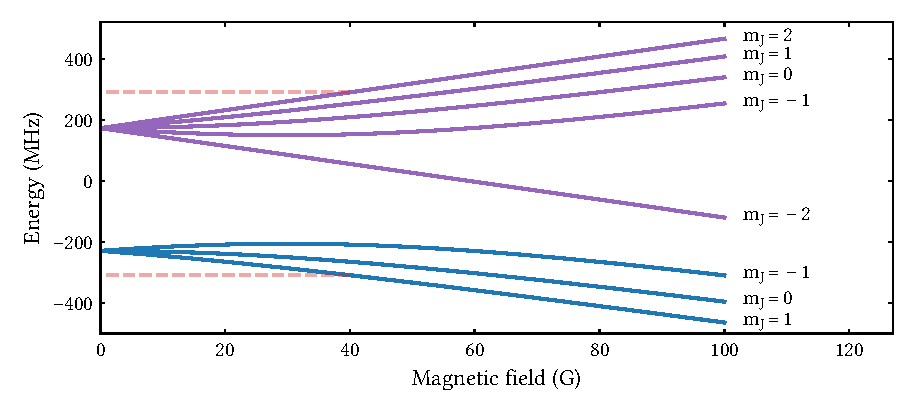
\includegraphics{figures/pot_zeeman_155.pdf}
\caption{The spectrum of ground state potassium is split into magnetic sublevels and shifted depending on a magnetic field applied to the atoms. Shown are two spin states $F=1$ in blue and $F=2$ in purple, relative to the ground state energy of $\ce{4S_{1/2}}$.}%
\label{fig:pot_zeeman}
}
\end{figure}


%As such, given generous, but realistic experimental parameters, it is apparent, that
%Although generous parameters were given for the calculation, we see that this approach would only work for very high magnetic fields.
The parameters used in the calculations are already on the optimistic end, which leads to the conclusion that this approach only works when very high magnetic fields are applied. Simulations show, that applying a magnetic field slope of $B=\SI{4000}{\gauss\per\centi\meter}$ results in a separation of $\SI{0.2}{\micro\meter}$. Luckily, there is another approach, which works by using only the light from frequency stable lasers, which is discussed in the following.

\begin{figure}[tbp]%
\centering{%
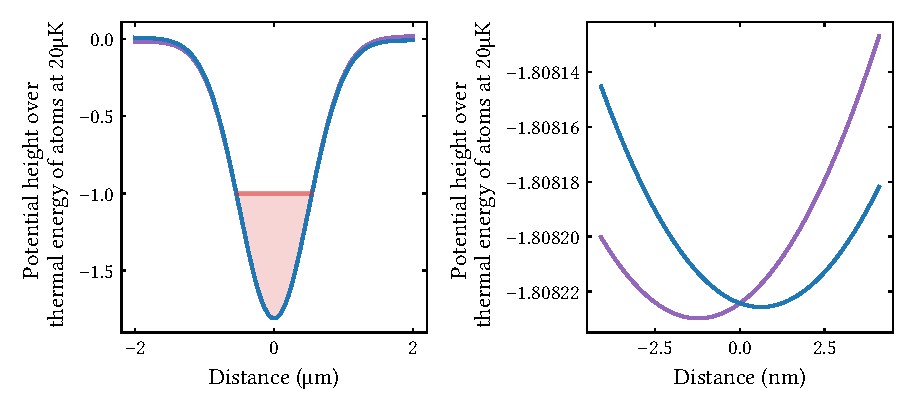
\includegraphics{figures/pot_separation_155.pdf}
\caption{Two spin species are subject to a dipole trap under the influence of a magnetic field gradient. The $F=1,m_F=1$ and $F=2,m_F=2$ states are colored in purple and blue respectively. The parameters for the trap are given in the text. Also shown is the energy of the atom as a red area. The zoomed in diagram on the right shows the separation of the two potentials, which is on the nanometer scale.}%
\label{fig:pot_separation}
}
\end{figure}

\subsection{Utilization of state selective light shifts}

There is another effect that affects the energy of the spin states, similar to the Zeeman effect, in which electrical fields also shift and split energy levels~\cite{Voigt, Courtney1995}. Under the influence of modulated electrical fields, such as coherent laser light, the effect is called AC Stark shift or simply light shift.

They are calculated in the semiclassical picture, where the light is treated classically and the atom is quantized. Moreover, in a simplified approach, the atom can be treated as a two-level system, when light is mostly resonant to a single excited state. Therefore, the electric field of the light and the state of the atom are written respectively as:

\begin{align}
	\mathbf{E}(\mathbf{r}, t) = \bm{\epsilon} E_0 \cos{(\mathbf{k r} - \omega_L t)} \\
	|\Psi \rangle = c_g(t) |g\rangle + c_e(t)|e\rangle.
\end{align}

Here, $\bm{\epsilon}$ is the electric field vector and $E_0$ its strength, $\bm{k}$ and $\omega_L$ are the wave vector and frequency of the field respectively. The state of the two-level atom changes with time, given by the ground and excited state probabilities $|c_g(t)|^2$ and $|c_e(t)|^2$. Moreover, the transition from the ground to the excited state has a resonance at $\omega_0$ and therefore the difference between the light frequency and the resonance is called the detuning, $\Delta = \omega_L - \omega_0$. The coupling between the electric field and the atom can be calculated from the dipole interaction and is simply $V_I = -\bm{\mu} \bm{E}$, given the dipole operator $\bm{\mu} = -e \bm{r}$. In this two-level system, where the atom is constantly driven by the electric field, the populations oscillate, however due to spontaneous emission, which can't be neglected, the excited state population will decay with time. This decay is calculated in~\cite{King2008} and the result is:

\begin{align}
	\label{eq:decay_rate}
	\Gamma = \frac{w_0^3}{3 \pi \epsilon_0 \hbar c^3} |\langle g | \bm{\mu} | e \rangle|^2.
\end{align}

To calculate the energy shift the states experience, perturbation theory can be applied in case the detuning is large~\cite{Grimm2000}, which to second order is in general:

\begin{align}
	\Delta E_i = \sum_{j\neq i} \frac{|\langle j| V_I | i \rangle|}{\epsilon_i - \epsilon_j}
\end{align}

Therefore, in the two-level system, the sum vanishes and the dipole matrix element $\langle e | \bm{\mu} | g \rangle$ can be replaced with the decay rate from Equation~\ref{eq:decay_rate} and therefore:

\begin{align}
	\Delta E_\pm = \pm \frac{|\langle e | \bm{\mu} | g \rangle|^2}{\Delta} |E^2| = \pm \frac{3 \pi c^2}{2 \omega_0^3} \frac{\Gamma}{\Delta} I
\end{align}

where the relation $I=2 \epsilon_0 c |E|^2$ was used. The plus and minus sign of the energy shift refer to the excited and ground states respectively and it can be seen, that these shifts only depend on the light field. The two-level system is only a simplification and in a more complete scenario, contributions from all excited states need to be summed up. Moreover, for large laser powers, coupling to the nuclear spin has to be considered, resulting in the hyperfine splitting of the energy levels~\cite{Grimm2000}. This results in the light shifts seen in Figure~\ref{fig:split_light_shift}, for the two spin states, $F=1$ and $F=2$ for the potassium atoms in the experiment.

\begin{figure}[tbp]%
	\centering{%
		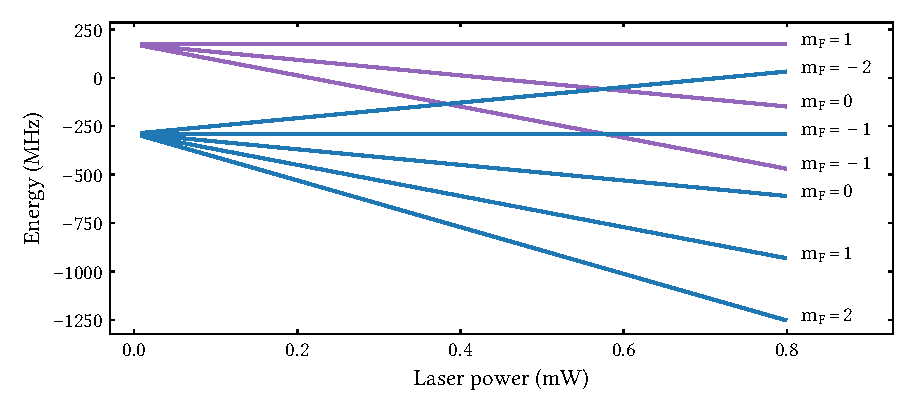
\includegraphics{figures/stark_shifts_155.pdf}
		\caption{The spin levels are split up due to the AC Stark shift from the laser illuminating the atoms. Shown are the ground states with $F=1$ in purple and $F=2$ in blue. The laser has a wavelength of $\SI{768.40}{\nano\meter}$ and positive circular polarization.}%
		\label{fig:split_light_shift}
	}%
\end{figure}%


Due to the light shifts, the atoms see an induced potential, given by the energy of the state. Therefore, the two spins can be spatially separated, when one component sees a potential, where the other one does not. This is easy to see in Figure~\ref{fig:light_shift_cross}, where the light shifts for the two spin states are given as a function of wavelength of the laser for circularly polarized light. We can see, that at $\SI{768.40}{\nano\meter}$, the $F=2$ state is trapped, while the $F=1$ component does not see a light shift, wich makes the atom with this spin transparent to the light.

\begin{figure}[tbp]%
\centering{%
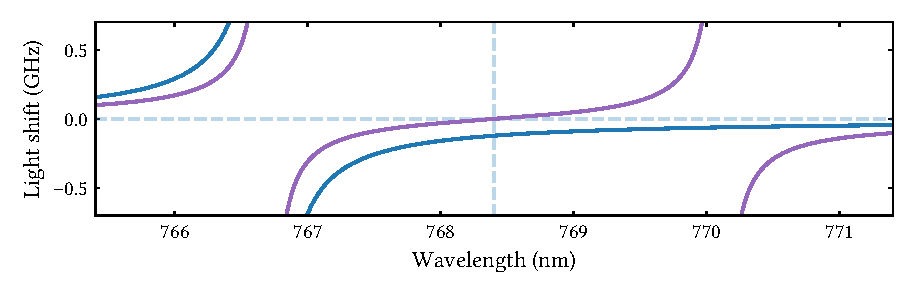
\includegraphics{figures/light_shift_cross_155.pdf}
\caption{The light shift of the $F=1,m_F=1$ (purple) and $F=2,m_F=2$ (blue) states against wavelength for a laser power of $\SI{0.1}{\milli\watt}$ and positive circular polarization. At $\SI{768.40}{\nano\meter}$, the $F=1$ component is transparent to the laser, therefore making it possible to trap only the $F=2$ state.}%
\label{fig:light_shift_cross}
}%
\end{figure}%

In the experiment then, the light is produced as optical tweezers using \acp{aod} as discussed in Chapter~\ref{sec:sorting} and mapped over the \ac{slm} tweezers. To transfer the atoms into the spin-selective tweezer, the resulting trap has to be much deeper than the initial tweezers. These have a power of $\approx\SI{15}{\milli\watt}$, but are highly detuned to the excited state on the D2 line at a wavelength of $\SI{1064}{\nano\meter}$. Moreover, high scattering rates will heat the atoms out of the trap and therefore, both of these quantities have been verified to be compatible with the experiment and are given in Figure~\ref{fig:relative_trap}. The trap depth of the spin-selective tweezer is almost twice as deep as the \ac{slm} tweezer for a laser power of $P=\SI{300}{\micro\watt}$, when the trap depth of the \ac{slm} tweezer is $\approx \SI{1}{\milli\kelvin}$. At this point, the scattering rate is $\Gamma_{sc} = \SI{2.5}{\kilo\hertz}$ or less than three photons per millisecond. Therefore, if the move happens during this time, almost no photons are being scattered. Moreover, a Raman sideband cooling technique that is implemented in the experiment~\cite{Thompson2013} allows to cool atoms even further, therefore trap depths can be reduced by at least a factor of ten, which reduces scattering over one millisecond to less than one. To verify, that heating is not an issue, the heating rate due to dipole traps has been calculated~\cite{Grimm2000} and is shown as a function of the laser power in Figure~\ref{fig:relative_trap} as well.
Consequently, using the AC-Stark shift in order to spatially separate the atoms is a viable approach to do spin-selective imaging.

%due to laser light having a bandwidth, the transparent spin might actually see a trap, therefore it needs to be verified, whether this effect is non-negligible. Figure~\ref{fig:relative_trap} shows the trap depth of the spin-sensitive tweezer over the trap depth of the initial tweezer, for both spin-species, when also accounting for a laser bandwidth of $\SI{100}{\giga\hertz}$. It turns out, that the bandwidth does not majorly affect the efficiency of not trapping the transparent state. Consequently, using the AC-Stark shift to shift atom levels is a viable approach in order to trap a single spin-component, allowing to image specific spin states.


\begin{figure}[tbp]%
\centering{%
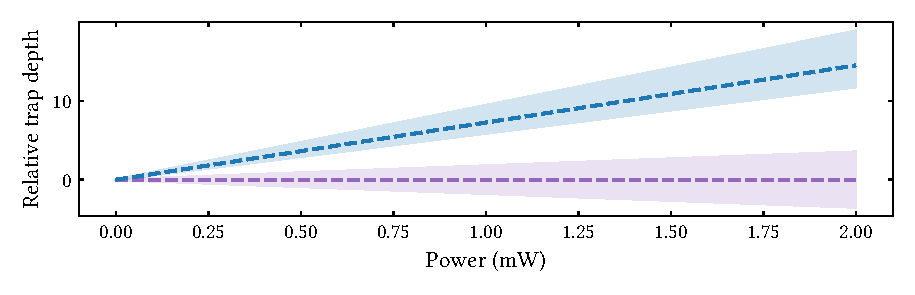
\includegraphics{figures/spin_rel_pot_155.pdf}
\caption{On the left, the relative trap depth between the spin-selective tweezer and the \ac{slm} tweezer is shown as a function of the spin-tweezer laser power. For the $F=1,m_F=1$ (purple) and $F=2,m_F=2$ (blue) state, only one state is trapped. Already at $\SI{0.3}{\milli\watt}$ power, the spin tweezer is more than 2 times deeper than the \ac{slm} tweezer. The shaded area is for reference if the laser is shifted by $\pm \SI{100}{\giga\hertz}$. The middle plot shows the scattering rate of the tweezer as a function of laser power, where both spin states scatter practically the same amount of photons. As a guide to the eye, the $\SI{0.3}{\milli\watt}$ power is shown as a dashed red line. In the same vein, the right plot shows the heating rate inside a harmonic potential.}%
\label{fig:relative_trap}
}
\end{figure}

\section{Setup}

We have seen, how light shifts can be used to trap a single spin species. Doing so, it is possible to spatially separate and image them onto a camera. However, it is necessary to have a stable laser at $\SI{768.40}{\nano\meter}$. The following section highlights the steps in order to build such a laser system, which includes setting up a cavity and a \ac{pdh} lock, that frequency stabilizes the system. The laser is then coupled into the same setup as in Chapter~\ref{sec:sorting}, allowing to generate acousto-optically deflected, spin-sensitive tweezers, allowing to move the spin state in space.

\subsection{Laser classification}

The laser classified in the following is a homebuilt model, the design of which is given in Appendix~\ref{ch:linear_laser}. It has room for a laser diode, whose light is collimated, filtered and reflected through a partially reflective mirror, which also serves as the output of the housing.
The laser diode (Eagleyard EYP-RWE-0760-02010-1500-SOT12-0000) used, is tunable in the range from $\SI{752}{\nano\meter}$ to $\SI{772}{\nano\meter}$ with a maximum power of $\SI{80}{\milli\watt}$. Since the diode is also used as the active medium, the cavity simplifies to being just a mirror, that reflects back into the diode and transmits part of the light out of the laser casing.

The laser power is classified as a function of current supplied to the laserdiode. Beyond the laser threshold, the power is linear with current and the diagram for the model built here is given in Figure~\ref{fig:laser_curve}.

%The light emitted from the laser device is then evaluated, based on the laser curve. This means, by increasing the current supplied to the laserdiode, there will be a point at which the power emitted from the cavity suddenly jumps. After that point, increasing the current on the laserdiode will increase the power in equal parts. This curve has been measured for the diode in question, verifying that the system is actually lasing, and is shown in Figure~\ref{fig:laser_curve}.

\begin{figure}[tbp]%
\centering{%
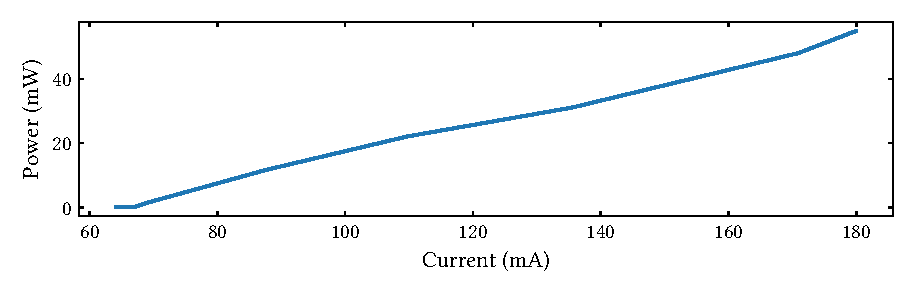
\includegraphics{figures/lasercurve_155.pdf}
\caption{Shown is the laser threshold for the home-built laser, driven with a Thorlabs LDC205C current controller. The power was measured using a Thorlabs PM100D power meter and the Thorlabs S121C sensor.}%
\label{fig:laser_curve}
}
\end{figure}

\subsection{Beam setup of spin-selective laser}

Now that there is a laser, the beam path in order to have a laser for spin-selective imaging can be set up. For this, two parts of the laser are split and coupled into fibers. One is used for monitoring of the wavelength, which will give an indication, if the frequency is currently locked or not. The second part will go to the cavity, allowing to actually perform the frequency stabilization. The full beam path is shown in Figure~\ref{fig:spin_beam_path}.

\begin{figure}[tbp]%
\centering{%
\import{figures}{setup_spin_laser.pdf_tex}
\caption{Shown is the setup, in order to prepare the spin-sensitive tweezer for the experiment. The laser first passes an isolator, in order to protect the laser cavity from reflections. It is then split into two paths for monitoring and frequency stabilization. An \ac{aod} is used to switch the light on and off for the experiment.}%
\label{fig:spin_beam_path}
}
\end{figure}

The main path is then coupled into a fibre, going towards the \ac{aod} discussed previously. However, the beam needs to be turned on and off at certain times during the experiment, for this, it first passes through an \ac{aom} and finally a shutter to block any leftover stray light. As shown previously, in~\ref{sec:tweezer_beams}, the light coming out of the fibre is then intensity stabilized and coupled into the \ac{aod}, which can be programmed to move the spin-sensitive tweezers.

\subsection{Cavity classification}

The laser has been built and characterized and can be coupled into the \ac{aod}, in order to generate movable tweezer for spin-selective imaging. However, the process requires a stable frequency at $\SI{768.40}{\nano\meter}$. As a matter of fact, not only are there resonances at $\SI{766.7}{\nano\meter}$ and $\SI{770.1}{\nano\meter}$, this spin-selecting procedure works by requires that one spin state is completely transparent to the laser light, in terms of seeing a dipole potential. In order to have the laser emit a stable frequency, a piezo tunes the position of the mirror inside the laser cavity based on an input signal. This way, the length of the cavity, and therefore the standing wave, can be selected. However, pressure and temperature can both affect the mirror, and therefore there needs to be a system in place, to compensate for these factors.

Consequently, it is necessary to have a device, that measures the instability, and feeds back a signal to the piezo. In order to do so, a part of the laser is split off and sent into a stable cavity. The light that has passed the cavity is measured using a photodiode and it is then possible to measure resonances of this cavity. With the \ac{pdh} method, an error signal is generated, that gives a feedback to the piezo. This generates a feedback loop, which is stable when the error signal is at a minimum. The process has been used and described in the experiment before~\cite{Hirthe2018}. The error signal recorded for this specific setup was recorded and is given in Chapter~\ref{ch:app_pdh}.
%When this is the case, a signal is generated, that is fed into the piezo, whenever the light on the photodiode is not on the resonance. This electronic signal is generated using the \acl{pdh} locking method and has been used and described in the experiment before~\cite{Hirthe2018}. An image of the \ac{pdh} from the cavity is given in Chapter~\ref{ch:app_pdh}.

The stable cavity in place for locking the laser frequency is made from a \ac{ule} glass, that has two mirrors attached to it. The material is not explicitly necessary, however the full extent of this specific \ac{ule} couldn't be used anymore, as only one side has the mirror contacted, while the other mirror is glued. Therefore, due to the glue, this cavity is still prone to some wavelength drifts, induced by temperature expanding and compressing the material. This specific application can deal with these instabilities and therefore the glass was recycled for this setup. In order to stabilize the cavity against temperature fluctuations, it rests in a copper housing. This copper housing further rests in a stainless steel container. This container is then evacuated with a vacuum pump, which stabilizes the cavity against pressure fluctuations. A picture of the cavity is given in Appendix~\ref{ch:app_cavity}.

In order to quantize the stability this cavity can provide, the frequency drift is measured. However, at $\SI{768.40}{\nano\meter}$, the frequency is in the hundreds of terahertz, which is difficult to measure conventionally. However, by superimposing a reference laser onto the spin-laser, that has a very stable frequency, it is possible to measure the beat note. Mathematically, this means adding two sine-signals together:

\begin{align}
	\sin{\left(2\pi f_1 t\right)} + \sin{\left( 2 \pi f_2 t \right)}
	= 2 \sin{\left( 2\pi \frac{f_1+f_2}{2}t \right)} \cos{\left( 2\pi \frac{f_1-f_2}{2}t \right)},
\end{align}

where $f_1$ and $f_2$ are the frequencies of the reference and spin-laser respectively.

This relation turns two modulations, which have the frequencies added and subtracted. The first one still can't be resolved, however if the difference frequency is low enough, it is possible to see it on a spectrum analyzer. This means, the frequency of the ``unstable'' laser was first matched to the stable laser, such that the difference frequency was at least in the Megahertz regime. Then, it is possible to observe the drift of the cavity, which is the change in frequency with time. This usually happens due to temperature drifts affecting the cavity. The measurement was taken over several days and recorded as in Figure~\ref{fig:cavity_drift}. Close to the end of the measurement, the drift was at a minimum of around $\SI{33}{\mega\hertz}$ per day, which is well within the limits, which can be verified with Figure~\ref{fig:relative_trap}. There, a shift of $\SI{100}{\giga\hertz}$ is shown as the shaded area and therefore it would take the cavity 30 days to drift to just one percent within this area. However it is important to note, that \ac{ule} glass has generally much lower drifts, on the order of kilohertz per day~\cite{Haindl2019}. This means, the glue on one side of the glass cavity is the limiting factor for these drifts and the only way to improve on this, is to replace the \ac{ule} glass.

With the cavity in place, all building blocks are there in order to separate spins of ground state potassium atoms. This means, the frequency stability given by the cavity locks the laser and makes it possible to position it close to the magic wavelength, where only one spin state sees a trap. By coupling the beam into the crossed \ac{aod}, each atom can be addressed and moved individually and an image of the spins can be acquired, while simultaneously keeping the atoms in the trap.

\begin{figure}[tbp]%
\centering{%
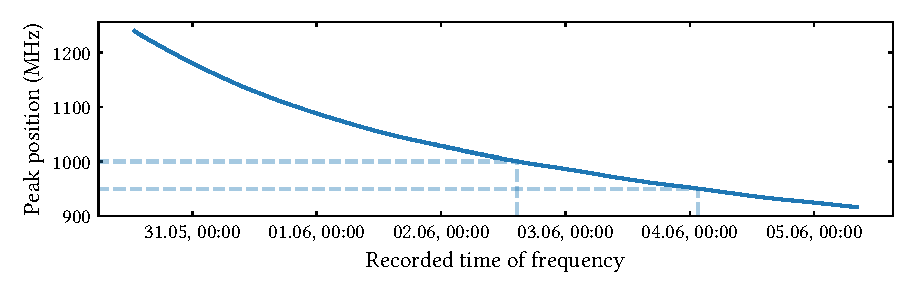
\includegraphics{figures/cavity_drift_155.pdf}
\caption{The cavity drift was recorded over six days by doing a beat measurement with a reference laser. Horizontal lines show $\SI{50}{\mega\hertz}$ difference at the end of the measurement, where temperature and pressure has stabilized. From this it can be seen, that the drift is on the order of $\SI{33}{\mega\hertz}$ per day.}%
\label{fig:cavity_drift}
}
\end{figure}
